\chapter{Robustness and Sensitivity}
\label{ch:robustness}

This chapter examines how far the results of Chapter~\ref{ch:results} depend on the choices made in the analysis and on chance. It starts with the inference (Section~\ref{sec:rob-bootstrap}), turns to the sample and the outcome (Section~\ref{sec:rob-sample}), to the way in which the transitions are summarised and to the baseline (Section~\ref{sec:rob-baseline}), and to the number of archetypes and the rate variables (Section~\ref{sec:rob-K}). Section~\ref{sec:rob-fuzziness} turns to the fuzziness of the memberships and the noise multiplier, Section~\ref{sec:rob-alignment} to the alignment of the archetypes, and Section~\ref{sec:rob-seeds} to the random draw of the clustering. Because many specifications are examined, $p$-values are not corrected unless stated, and the pattern across specifications is more informative than any single value. The main configuration of Chapter~\ref{ch:results} remains the reference throughout.

\section{Estimated memberships: the bootstrap}
\label{sec:rob-bootstrap}

Table~\ref{tab:bootstrap-K} compares the conventional Wald tests, which treat the memberships as observed, with the tests based on the two-stage bootstrap (Section~\ref{sec:method-bootstrap}) for the main fuzziness and noise settings ($m=1.3$, $\rho=1.0$) and different numbers of archetypes and rate variables. The bootstrap standard errors are larger than the conventional ones by 7 to 46\% depending on the cell and the baseline, 19\% on average, and the correction is largest where the memberships are least reliable: for $K=3$ with shrunk rates it raises the $p$-value of the core test from 0.27 to 0.56 and that of the full test from 0.05 to 0.34. For the main configuration the ratio is 1.08 and 1.15, and the joint $p$-values change from 0.027 to 0.079 and from 0.002 to 0.015, so the correction matters for the conclusion: against the core baseline the association is no longer significant at 5\%. The mean of the bootstrap estimates also differs from the original coefficients, by up to 0.17 for individual coefficients in the settings reported below and in the direction of zero in the cases with the largest differences, as would be expected if noise in the memberships attenuated the coefficients. The bootstrap corrects the standard errors but not this attenuation, so the point estimates should be read as conservative.

\begin{table}[ht]
	\centering
	\small
	\caption{Conventional and bootstrap tests by number of archetypes and rate variables ($m=1.3$, $\rho=1.0$)}
	\label{tab:bootstrap-K}
	\begin{tabular}{llrrrrrrr}
		\toprule
		 & & \multicolumn{2}{c}{Core: $p$} & \multicolumn{2}{c}{Full: $p$} & SE & \multicolumn{2}{c}{Full baseline} \\
		\cmidrule(lr){3-4}\cmidrule(lr){5-6}\cmidrule(lr){8-9}
		Rates & $K$ & Conv. & Boot. & Conv. & Boot. & ratio & $\Delta\bar R^2$ & $\Delta R^2_{oos}$ \\
		\midrule
Shrunk & 3 & 0.266 & 0.557 & 0.053 & 0.335 & 1.40 & +0.17 & +0.01 \\
Shrunk & 4 & 0.027 & 0.079 & 0.002 & 0.015 & 1.11 & +0.56 & +0.33 \\
Shrunk & 5 & 0.428 & 0.723 & 0.522 & 0.757 & 1.30 & -0.02 & -0.25 \\
Raw & 3 & 0.054 & 0.077 & 0.003 & 0.012 & 1.10 & +0.58 & +0.47 \\
Raw & 4 & 0.034 & 0.055 & 0.002 & 0.016 & 1.17 & +0.59 & +0.40 \\
		\bottomrule
	\end{tabular}
	\par\smallskip
	\parbox{0.95\textwidth}{\footnotesize\emph{Note.} Wald $p$-values of the block of membership changes with cluster-robust (conventional) and bootstrap covariance matrices (500 replications). SE ratio is the average over both baselines of the mean ratio of the bootstrap to the conventional standard errors. $\Delta\bar R^2$ and $\Delta R^2_{oos}$ are the gains in adjusted and cross-validated $R^2$ against the full baseline, in percentage points. The row for shrunk rates and $K=4$ is the main configuration.}
\end{table}

\section{Sample and outcome}
\label{sec:rob-sample}

The association in the main configuration is not driven by the definition of the sample or the outcome (Table~\ref{tab:variations}). Against the full baseline, the block of membership changes is significant at 5\% in seven of the eight variations, and against the core baseline in five of eight, with changes in the adjusted $R^2$ that are positive in all of them (0.09 to 0.39 percentage points for the core baseline and 0.23 to 0.56 for the full baseline). The exceptions are the sample without the pandemic seasons (960 pairs), against both baselines, the players who did not change club (1,058 pairs) against the core baseline ($p=0.24$; the full-baseline test is just significant at $p=0.046$), and the players aged up to 30 against the core baseline ($p=0.064$): in these the gains stay positive but the tests lose power. The result is the same with player fixed effects (Section~\ref{sec:results-valuation}). These variations and the fixed-effects comparison were computed for the main configuration only, with conventional standard errors.

\begin{table}[ht]
	\centering
	\small
	\caption{Sample and outcome variations (main configuration)}
	\label{tab:variations}
	\begin{tabular}{lrrrrrr}
		\toprule
		 & & & \multicolumn{2}{c}{Core baseline} & \multicolumn{2}{c}{Full baseline} \\
		\cmidrule(lr){4-5}\cmidrule(lr){6-7}
		Variation & Pairs & Players & $p$ & $\Delta\bar R^2$ & $p$ & $\Delta\bar R^2$ \\
		\midrule
All pairs (main configuration) & 1,361 & 697 & 0.027 & +0.34 & 0.002 & +0.56 \\
Winsorised outcome (1st and 99th percentile) & 1,361 & 697 & 0.033 & +0.30 & 0.004 & +0.50 \\
Players who did not change club & 1,058 & 611 & 0.240 & +0.09 & 0.046 & +0.23 \\
Non-zero changes in value only & 1,164 & 632 & 0.047 & +0.31 & 0.010 & +0.46 \\
At least 500 minutes in both seasons & 1,069 & 574 & 0.023 & +0.39 & 0.015 & +0.44 \\
Without pairs starting in 2019/20 and 2020/21 & 960 & 598 & 0.270 & +0.16 & 0.158 & +0.23 \\
Players aged 30 or younger & 1,222 & 642 & 0.064 & +0.28 & 0.007 & +0.52 \\
Without noise-dominated players (noise membership $>0.5$) & 1,283 & 669 & 0.035 & +0.33 & 0.009 & +0.49 \\
		\bottomrule
	\end{tabular}
	\par\smallskip
	\parbox{0.95\textwidth}{\footnotesize\emph{Note.} Cluster-robust Wald $p$-values of the block of membership changes; $\Delta\bar R^2$ is the change in adjusted $R^2$ in percentage points.}
\end{table}

\section{Summaries of the transitions and the baseline}
\label{sec:rob-baseline}

\paragraph{Direction, size and specialisation.} Replacing the membership changes by the size of the shift or by the change in entropy removes the association in the main configuration (Table~\ref{tab:comparison}), and so does adding the membership levels at the start of the season. What is associated with the change in value is the direction of the movement.

\paragraph{Linear summaries.} Principal component scores condense the same twelve statistics linearly. The first four components explain about 71\% of their variance. Their changes are jointly insignificant against the core baseline ($p=0.48$, change in adjusted $R^2$ of $-0.01$ percentage points), and so are those of the first eight ($p=0.59$). They cannot be tested against the full baseline, which already contains the changes of every statistic. This benchmark does not depend on $m$ or on the random draw. Because the membership changes are significant at several values of $m$ (Section~\ref{sec:rob-fuzziness}) where the linear summary is not, any association that the memberships carry is not a reflection of linear changes in the performance statistics.

\paragraph{Controls without performance statistics.} The overlap between the memberships and the performance controls is the reason for the full baseline, and the opposite check removes the performance controls altogether. A baseline with only age, playing time, position, team form, club change and season effects has an adjusted $R^2$ of 0.433, compared with 0.448 once goals and assists are added. Table~\ref{tab:minimal} shows that the membership changes do not behave differently against this baseline: they are significant at $m=1.3$ ($p=0.020$) and more clearly at $m=1.4$ and $m=1.5$ ($p=0.001$ and $p<0.001$ with conventional standard errors), with gains in out-of-sample $R^2$ of 0.44 and 0.59 percentage points at these two values. The membership changes are therefore not proxies for goals and assists.

\begin{table}[ht]
	\centering
	\small
	\caption{Benchmarks for the membership changes}
	\label{tab:minimal}
	\begin{tabular}{lrrr}
		\toprule
		\multicolumn{4}{l}{\emph{A. Principal component scores against the core baseline}} \\
		 & $p$ & $\Delta\bar R^2$ & $\Delta R^2_{oos}$ \\
		\midrule
Principal components, first 4 & 0.483 & -0.01 & --- \\
Principal components, first 8 & 0.589 & +0.00 & --- \\
		\midrule
		\multicolumn{4}{l}{\emph{B. Membership changes against the baseline without performance statistics}} \\
		Fuzziness $m$ & $p$ & $\Delta\bar R^2$ & $\Delta R^2_{oos}$ \\
		\midrule
1.2 & 0.108 & +0.26 & -0.04 \\
1.3 & 0.020 & +0.39 & +0.13 \\
1.4 & 0.001 & +0.63 & +0.44 \\
1.5 & 0.000 & +0.74 & +0.59 \\
2.0 & 0.005 & +0.53 & +0.36 \\
		\bottomrule
	\end{tabular}
	\par\smallskip
	\parbox{0.95\textwidth}{\footnotesize\emph{Note.} Cluster-robust Wald $p$-values, treating the memberships as observed; changes in adjusted and cross-validated $R^2$ in percentage points. Panel B: shrunk rates, $K=4$, $\rho=1.0$. $N=1{,}361$.}
\end{table}

\section{Number of archetypes and rate variables}
\label{sec:rob-K}

At $m=1.3$ the number of archetypes and the treatment of the rates matter more than the sample (Table~\ref{tab:bootstrap-K}). With the bootstrap, three of the ten tests are below 5\% (shrunk rates with $K=4$, raw rates with $K=3$ and raw rates with $K=4$, all against the full baseline), three more lie between 5 and 8\% (all against the core baseline), and the other four are well above. With shrunk rates, $K=3$ and $K=5$ show no association (bootstrap $p$-values of 0.34 and 0.76 against the full baseline); with raw rates, $K=3$ and $K=4$ do. The gains are small: where the full-baseline test is significant, the adjusted $R^2$ rises by 0.56 to 0.59 percentage points and the out-of-sample $R^2$ by 0.33 to 0.47 points. The association is therefore not specific to the shrunk rates, which also appears in the specification grid below, but it is specific to some numbers of archetypes, and $K=5$ stands out as the setting in which it is most often absent (Table~\ref{tab:grid}).

\section{Fuzziness and the noise multiplier}
\label{sec:rob-fuzziness}

The fuzziness exponent $m$ is the setting on which the results depend most. Table~\ref{tab:fuzziness} fixes the other settings of the main configuration and varies $m$ from 1.2 to 2.0. Larger values of $m$ spread the memberships more evenly, as the column on crispness shows: the share of players with a largest membership of at least 0.7 falls from 76\% at $m=1.2$ to 63\% at $m=1.3$ (the main configuration), 49\% at $m=1.4$, 37\% at $m=1.5$ and 4\% at $m=2.0$, where the memberships are almost uniform and hardly describe archetypes. The noise share rises from 4.8\% to 12\%, and the persistence of archetypes is between 0.67 and 0.75 for $m$ from 1.2 to 1.5 and falls to 0.54 at $m=2.0$.

\begin{table}[ht]
	\centering
	\footnotesize
	\setlength{\tabcolsep}{3.5pt}
	\caption{Sensitivity to the fuzziness exponent $m$ (shrunk rates, $K=4$, $\rho=1.0$)}
	\label{tab:fuzziness}
	\begin{tabular}{rrrrrrrrrrr}
		\toprule
		 & & & & & \multicolumn{3}{c}{Core baseline} & \multicolumn{3}{c}{Full baseline} \\
		\cmidrule(lr){6-8}\cmidrule(lr){9-11}
		$m$ & Crisp & Noise & Persist. & XB & $p$ & $\Delta\bar R^2$ & $\Delta R^2_{oos}$ & $p$ & $\Delta\bar R^2$ & $\Delta R^2_{oos}$ \\
		\midrule
1.2 & 76\% & 4.8\% & 0.71 & 0.89 & 0.445 & +0.09 & -0.22 & 0.277 & +0.18 & -0.07 \\
1.3 & 63\% & 5.3\% & 0.75 & 0.72 & 0.079 & +0.34 & +0.13 & 0.015 & +0.56 & +0.43 \\
1.4 & 49\% & 6.3\% & 0.70 & 0.66 & 0.037 & +0.42 & +0.28 & 0.008 & +0.66 & +0.58 \\
1.5 & 37\% & 7.3\% & 0.67 & 0.75 & 0.029 & +0.52 & +0.41 & 0.008 & +0.75 & +0.72 \\
2.0 & 4\% & 12.0\% & 0.54 & 0.63 & 0.088 & +0.22 & +0.06 & 0.019 & +0.43 & +0.25 \\
		\bottomrule
	\end{tabular}
	\par\smallskip
	\parbox{0.95\textwidth}{\footnotesize\emph{Note.} Crisp is the share of players whose largest substantive membership is at least 0.7; Noise the share assigned to the noise cluster; Persist.\ the share who keep their archetype; XB the Xie--Beni index averaged over seasons (lower is better). $p$ is the bootstrap Wald $p$-value of the block of membership changes (500 replications); $\Delta\bar R^2$ and $\Delta R^2_{oos}$ are gains in adjusted and cross-validated $R^2$ in percentage points (ten cross-validation repetitions, so the row $m=1.3$ differs slightly from Table~\ref{tab:comparison}, which uses 30). The row $m=1.3$ is the main configuration.}
\end{table}

With near-crisp memberships ($m=1.2$) there is no association after the bootstrap ($p=0.45$ and $0.28$). From $m=1.3$ on the membership changes are jointly significant against the full baseline ($p=0.015$, $0.008$, $0.008$ and $0.019$ at $m=1.3$, 1.4, 1.5 and 2.0), and against the core baseline they are significant at $m=1.4$ and $m=1.5$ ($p=0.037$ and $0.029$) and borderline at $m=1.3$ and $m=2.0$ ($p=0.079$ and $0.088$). The adjusted $R^2$ rises by 0.4 to 0.5 percentage points against the core baseline and by 0.7 to 0.8 points against the full baseline at $m=1.4$ and $1.5$, and the out-of-sample $R^2$ by 0.3 to 0.4 and by 0.6 to 0.7 points. The values $m=1.4$ and $m=1.5$ lie within the range of 1 to 1.5 that is recommended for medoid-based methods, and $m=1.5$ is one of the three values compared by \citeA{durso2022robust}. Within the main configuration the Xie--Beni index is lowest at $m=1.4$ among the values from 1.2 to 1.5, which is the value that the proposal's selection rule would have chosen; this was not the rule used (Chapter~\ref{ch:methodology}), but the reader should know that the results at that value are somewhat stronger than in the main configuration.

The archetypes are the same types at $m=1.3$, $1.4$ and $1.5$. The medoids are defenders in all eight seasons for one archetype, forwards for the strikers, forwards with a midfield role for the wide attackers, and midfielders for the central midfielders. The numbering of the archetypes differs between runs, because it is inherited from the first season, so coefficients are compared by the type of archetype. In all three runs the reference is the defenders and all coefficients are negative, and the one that stands out is that of the wide attackers: $-0.22$ and $-0.31$ against the core and full baselines at $m=1.3$, $-0.26$ and $-0.36$ at $m=1.4$ (bootstrap $p=0.004$ and $0.001$), and $-0.31$ and $-0.41$ at $m=1.5$ ($p=0.003$ and $0.001$). The shift from the defender profile to the wide-attacker profile is therefore the association that is found, and it grows in size with the fuzziness. A shift of 0.10 corresponds to a difference in value of about $-2$ to $-3$ per cent at $m=1.3$ and about $-3$ to $-4$ per cent at $m=1.5$.

\paragraph{Noise multiplier.} A lower noise multiplier ($\rho=0.75$) increases the noise share to 14\% and a higher one ($\rho=1.5$) lowers it to 1.5\%. At $m=1.3$ the conventional $p$-values are 0.046 (core) and 0.002 (full) at $\rho=0.75$, 0.027 and 0.002 at the main value $\rho=1.0$, and 0.099 and 0.014 at $\rho=1.5$; with the bootstrap, $\rho=1.5$ gives 0.171 and 0.069. The association is therefore weaker when fewer players are put into the noise cluster.

\paragraph{The whole specification space.} Table~\ref{tab:grid} summarises the 120 combinations of rates, number of archetypes, noise multiplier and fuzziness, and Figure~\ref{fig:grid} shows the conventional $p$-values. Against the core baseline, 34 of the 120 specifications (28\%) have a $p$-value below 5\%; against the full baseline 74 (62\%) do. The adjusted $R^2$ increases in 92 (core) and 107 (full) of the specifications, by a median of 0.13 and 0.28 percentage points and by at most 0.83 points. The out-of-sample $R^2$ increases in 43 (core) and 79 (full) of the 120 specifications, with medians of $-0.08$ and $+0.13$ points and a maximum of 0.72 points. The proportion of significant results is highest at $K=4$ (53\% core, 83\% full) and lowest at $K=5$ (10\% and 30\%), highest at $m=1.5$ (38\% core, 83\% full) and, against the full baseline, lowest at $m=1.2$ (42\%) and $m=2.0$ (50\%). It is the same for shrunk and raw rates against the core baseline (28\% each) and somewhat higher for raw rates against the full baseline (70\% against 53\%). The map in Figure~\ref{fig:grid} is patchy and not a smooth function of $m$ and $K$, which suggests that part of the pattern reflects the idiosyncrasies of individual clustering solutions and of the random draw (Section~\ref{sec:rob-seeds}).

\begin{table}[ht]
	\centering
	\small
	\caption{Summary of the specification grid (120 specifications)}
	\label{tab:grid}
	\begin{tabular}{lrrrrrrr}
		\toprule
		 & & \multicolumn{2}{c}{Share with $p<0.05$} & \multicolumn{2}{c}{Median $\Delta\bar R^2$} & \multicolumn{2}{c}{Median $\Delta R^2_{oos}$} \\
		\cmidrule(lr){3-4}\cmidrule(lr){5-6}\cmidrule(lr){7-8}
		 & $N$ & Core & Full & Core & Full & Core & Full \\
		\midrule
All specifications & 120 & 28\% & 62\% & +0.13 & +0.28 & -0.08 & +0.13 \\
\midrule
\multicolumn{8}{l}{\emph{By fuzziness $m$}} \\
\quad $m=1.2$ & 24 & 25\% & 42\% & +0.07 & +0.17 & -0.15 & -0.04 \\
\quad $m=1.3$ & 24 & 17\% & 67\% & +0.16 & +0.37 & -0.09 & +0.17 \\
\quad $m=1.4$ & 24 & 38\% & 67\% & +0.13 & +0.35 & -0.07 & +0.20 \\
\quad $m=1.5$ & 24 & 38\% & 83\% & +0.18 & +0.47 & -0.07 & +0.20 \\
\quad $m=2.0$ & 24 & 25\% & 50\% & +0.10 & +0.19 & -0.08 & +0.02 \\
\midrule
\multicolumn{8}{l}{\emph{By number of archetypes $K$}} \\
\quad $K=3$ & 30 & 23\% & 67\% & +0.12 & +0.26 & -0.01 & +0.17 \\
\quad $K=4$ & 30 & 53\% & 83\% & +0.20 & +0.40 & +0.04 & +0.26 \\
\quad $K=5$ & 30 & 10\% & 30\% & +0.01 & +0.12 & -0.17 & -0.09 \\
\quad $K=6$ & 30 & 27\% & 67\% & +0.17 & +0.37 & -0.10 & +0.10 \\
\midrule
\multicolumn{8}{l}{\emph{By noise multiplier $\rho$}} \\
\quad $\rho=0.75$ & 40 & 28\% & 70\% & +0.14 & +0.31 & -0.06 & +0.18 \\
\quad $\rho=1.0$ & 40 & 22\% & 50\% & +0.07 & +0.22 & -0.10 & +0.06 \\
\quad $\rho=1.5$ & 40 & 35\% & 65\% & +0.13 & +0.27 & -0.07 & +0.10 \\
\midrule
\multicolumn{8}{l}{\emph{By rate variables}} \\
\quad Shrunk & 60 & 28\% & 53\% & +0.13 & +0.23 & -0.08 & +0.08 \\
\quad Raw & 60 & 28\% & 70\% & +0.13 & +0.34 & -0.09 & +0.16 \\
		\bottomrule
	\end{tabular}
	\par\smallskip
	\parbox{0.95\textwidth}{\footnotesize\emph{Note.} Specifications combine shrunk or raw rates, $K\in\{3,4,5,6\}$, $\rho\in\{0.75,1.0,1.5\}$ and $m\in\{1.2,1.3,1.4,1.5,2.0\}$. $p$-values are conventional cluster-robust Wald tests and treat the memberships as observed. Gains in adjusted and cross-validated $R^2$ (ten repetitions) are in percentage points. $N$ is the number of specifications in the row.}
\end{table}

\begin{figure}[ht]
	\centering
	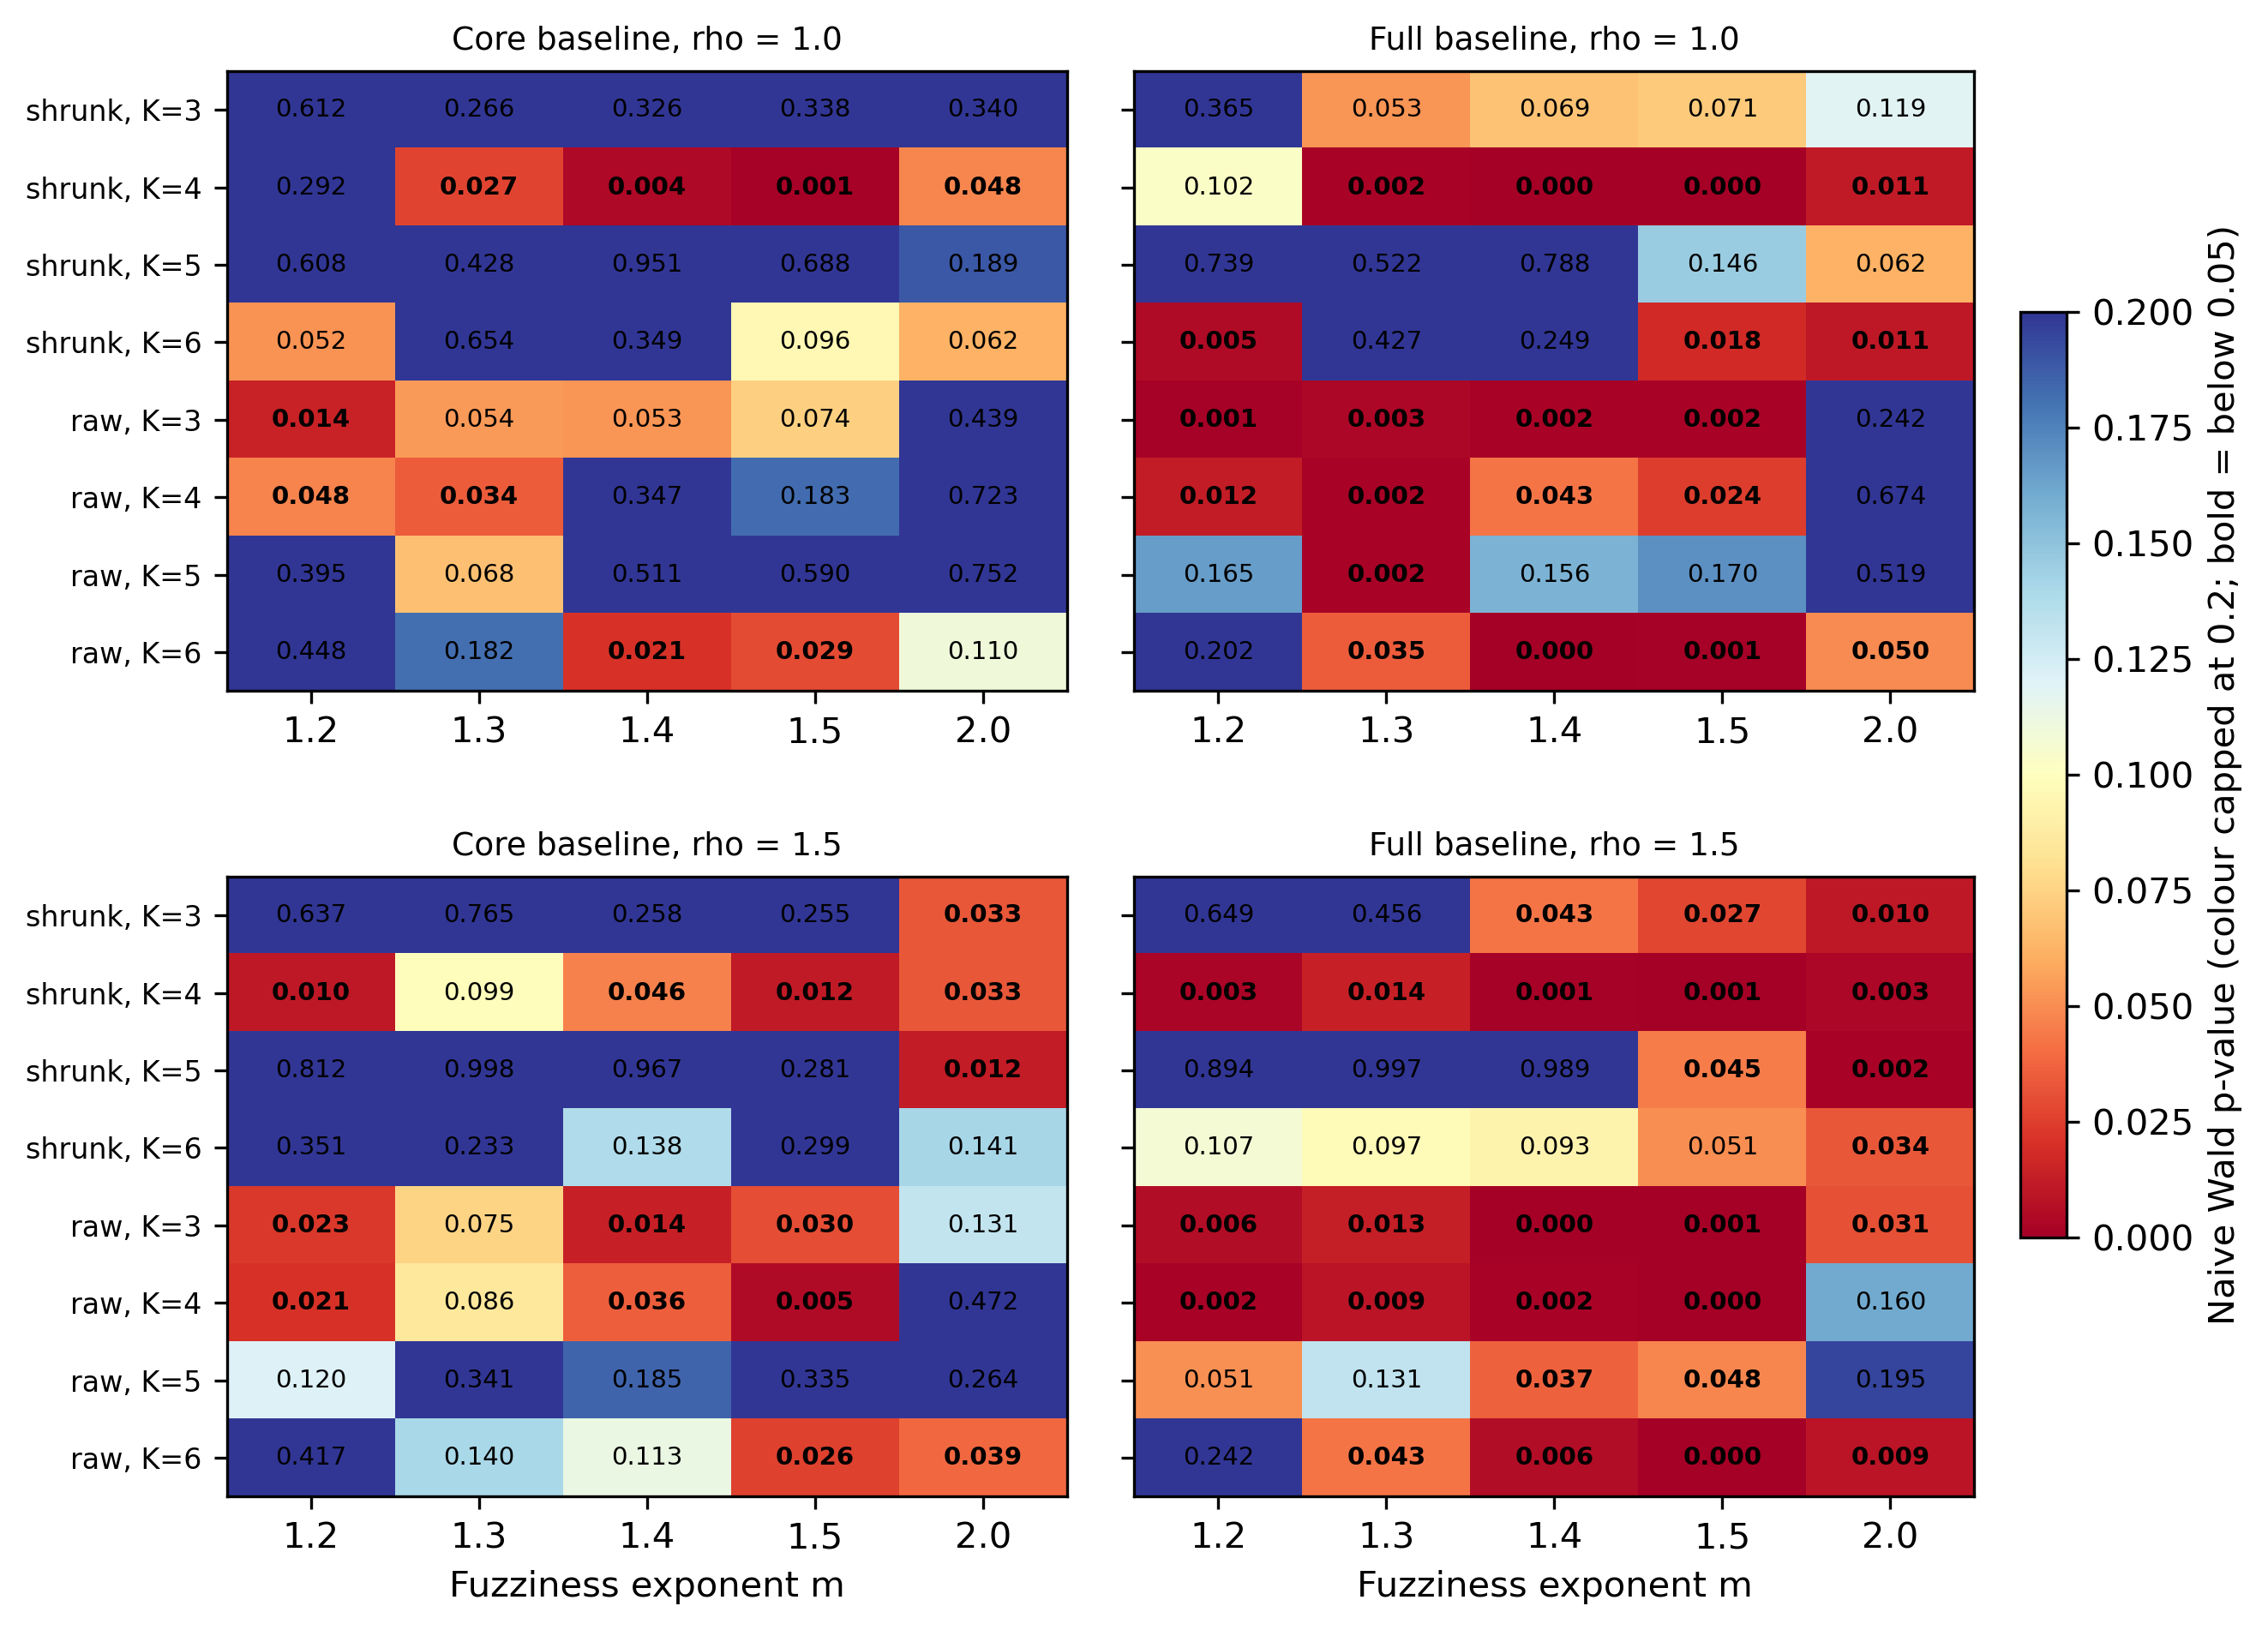
\includegraphics[width=\textwidth]{thesis_outputs/figures/spec_heatmap.png}
	\caption{Conventional Wald $p$-values across the specification grid}
	\label{fig:grid}
	\par\smallskip
	\parbox{0.95\textwidth}{\footnotesize\emph{Note.} Each cell is one specification. Colour is capped at $p=0.2$; bold values are below 0.05. The left panels use the core baseline, the right panels the full baseline; the upper panels $\rho=1.0$ and the lower panels $\rho=1.5$.}
\end{figure}

\paragraph{Multiple comparisons.} The bootstrap was applied to twenty comparisons (ten configurations against two baselines). The smallest bootstrap $p$-value is 0.0076. Neither if the ten comparisons of the fuzziness grid are treated as one family nor if all twenty are does any comparison survive a Holm correction at the 5\% level, since the thresholds are 0.005 and 0.0025. The specifications are not independent tests of different hypotheses, which makes this correction conservative, but it shows that the evidence is not strong enough to rely on any single cell.

\section{Consistency of the archetype labels across seasons}
\label{sec:rob-alignment}

The alignment of the archetypes across seasons determines whether a change in a membership is a real transition. The first version of the analysis matched archetypes by the distance between medoids. Its quality was checked for every one of the 120 clustering runs of the specification grid with information that the matching does not use: the profiles of the archetypes. For each pair of adjacent seasons, the check asks whether label $k$ in season $t$ is matched to label $k$ in season $t+1$ when the profiles are matched optimally; a pair is inconsistent if not.

The check found consistent labels in every season pair in only 36 of the 120 runs (30\%). The share falls steeply with the number of clusters: 73\% for $K=3$, 27\% for $K=4$, 17\% for $K=5$ and 3\% for $K=6$. For the shrunk-rate runs with $K=4$ and $\rho=1.0$ it was consistent at $m=1.3$ (the main configuration) and $m=1.4$, and inconsistent in one season pair at $m=1.5$ (2022/23 to 2023/24), in two at $m=2.0$ and in three at $m=1.2$. The inconsistency at $m=1.5$ agrees with what the medoids showed: the central-midfielder and striker medoids of 2023/24 and 2024/25 appeared under the numbers that held other archetypes earlier. For this reason the alignment uses the profiles of the archetypes (Section~\ref{sec:method-alignment}), and \emph{all results in Chapters~\ref{ch:results} and~\ref{ch:robustness}, including the specification grid and the bootstrap, were recomputed with this alignment}. This is a correction of the method made because of the label check and not because of any outcome. After the correction, the labels are consistent in all 120 runs by construction; the independent check is the position labels of the medoids, which do not enter the alignment. The share of seasons in which an archetype's medoid has the archetype's most common position label is 0.88 at $m=1.2$ and $1.3$, 0.84 at $m=1.4$, 0.75 at $m=1.5$ and 0.59 at $m=2.0$ in the $K=4$ runs with shrunk rates, and between 0.74 and 0.79 on average for each $K$ over all runs. The archetypes are thus well defined at $m\le1.4$ and less so at $m=1.5$ and $m=2.0$, where the memberships are softer.

\section{The random draw of the clustering}
\label{sec:rob-seeds}

The clustering starts from random medoids, and the partitions of different starts agree only moderately (an adjusted Rand index of about 0.5, Table~\ref{tab:selection}). The best of ten starts is kept for every season, but the objective is flat, so that another seed, or another ordering of the rows, can yield different memberships and different test results. This was seen directly: a run of the same main configuration made before the correction of the alignment and of the data (the data correction is described in Chapter~\ref{ch:data}), with a different ordering of the rows, gave conventional $p$-values of 0.70 (core) and 0.36 (full), against 0.027 and 0.002 in the run reported in Chapter~\ref{ch:results}. To measure the dependence on the draw, the first stage (the clustering of all seasons and the alignment) was repeated with 30 different seeds for each fuzziness value, and the key test was repeated each time (Table~\ref{tab:seeds}, Figure~\ref{fig:seeds}).

\begin{table}[ht]
	\centering
	\footnotesize
	\setlength{\tabcolsep}{3pt}
	\caption{Results over 30 random draws of the clustering (shrunk rates, $K=4$, $\rho=1.0$)}
	\label{tab:seeds}
	\resizebox{\textwidth}{!}{%
	\begin{tabular}{rrrrrrrrrrr}
		\toprule
		 & \multicolumn{2}{c}{Core baseline} & \multicolumn{4}{c}{Full baseline} & \multicolumn{2}{c}{Median $\Delta\bar R^2$} & \multicolumn{2}{c}{Median $\Delta R^2_{oos}$} \\
		\cmidrule(lr){2-3}\cmidrule(lr){4-7}\cmidrule(lr){8-9}\cmidrule(lr){10-11}
		$m$ & Median $p$ & $p<0.05$ & Median $p$ & IQR & Max & $p<0.05$ & Core & Full & Core & Full \\
		\midrule
1.2 & 0.224 & 17\% & 0.086 & 0.008--0.145 & 0.50 & 40\% & +0.05 & +0.22 & -0.15 & +0.03 \\
1.3 & 0.113 & 37\% & 0.025 & 0.004--0.083 & 0.32 & 60\% & +0.13 & +0.26 & -0.07 & +0.12 \\
1.4 & 0.082 & 37\% & 0.008 & 0.002--0.070 & 0.31 & 67\% & +0.14 & +0.38 & -0.02 & +0.23 \\
1.5 & 0.101 & 27\% & 0.016 & 0.005--0.051 & 0.55 & 73\% & +0.10 & +0.33 & -0.07 & +0.17 \\
2.0 & 0.266 & 17\% & 0.093 & 0.015--0.192 & 0.88 & 43\% & +0.04 & +0.15 & -0.11 & +0.04 \\
		\bottomrule
	\end{tabular}}
	\par\smallskip
	\parbox{0.95\textwidth}{\footnotesize\emph{Note.} Conventional cluster-robust Wald $p$-values of the block of membership changes; $p<0.05$ is the share of draws in which the test is significant; IQR is the interquartile range of the $p$-values; gains in adjusted and cross-validated $R^2$ (ten repetitions) are medians in percentage points.}
\end{table}

\begin{figure}[ht]
	\centering
	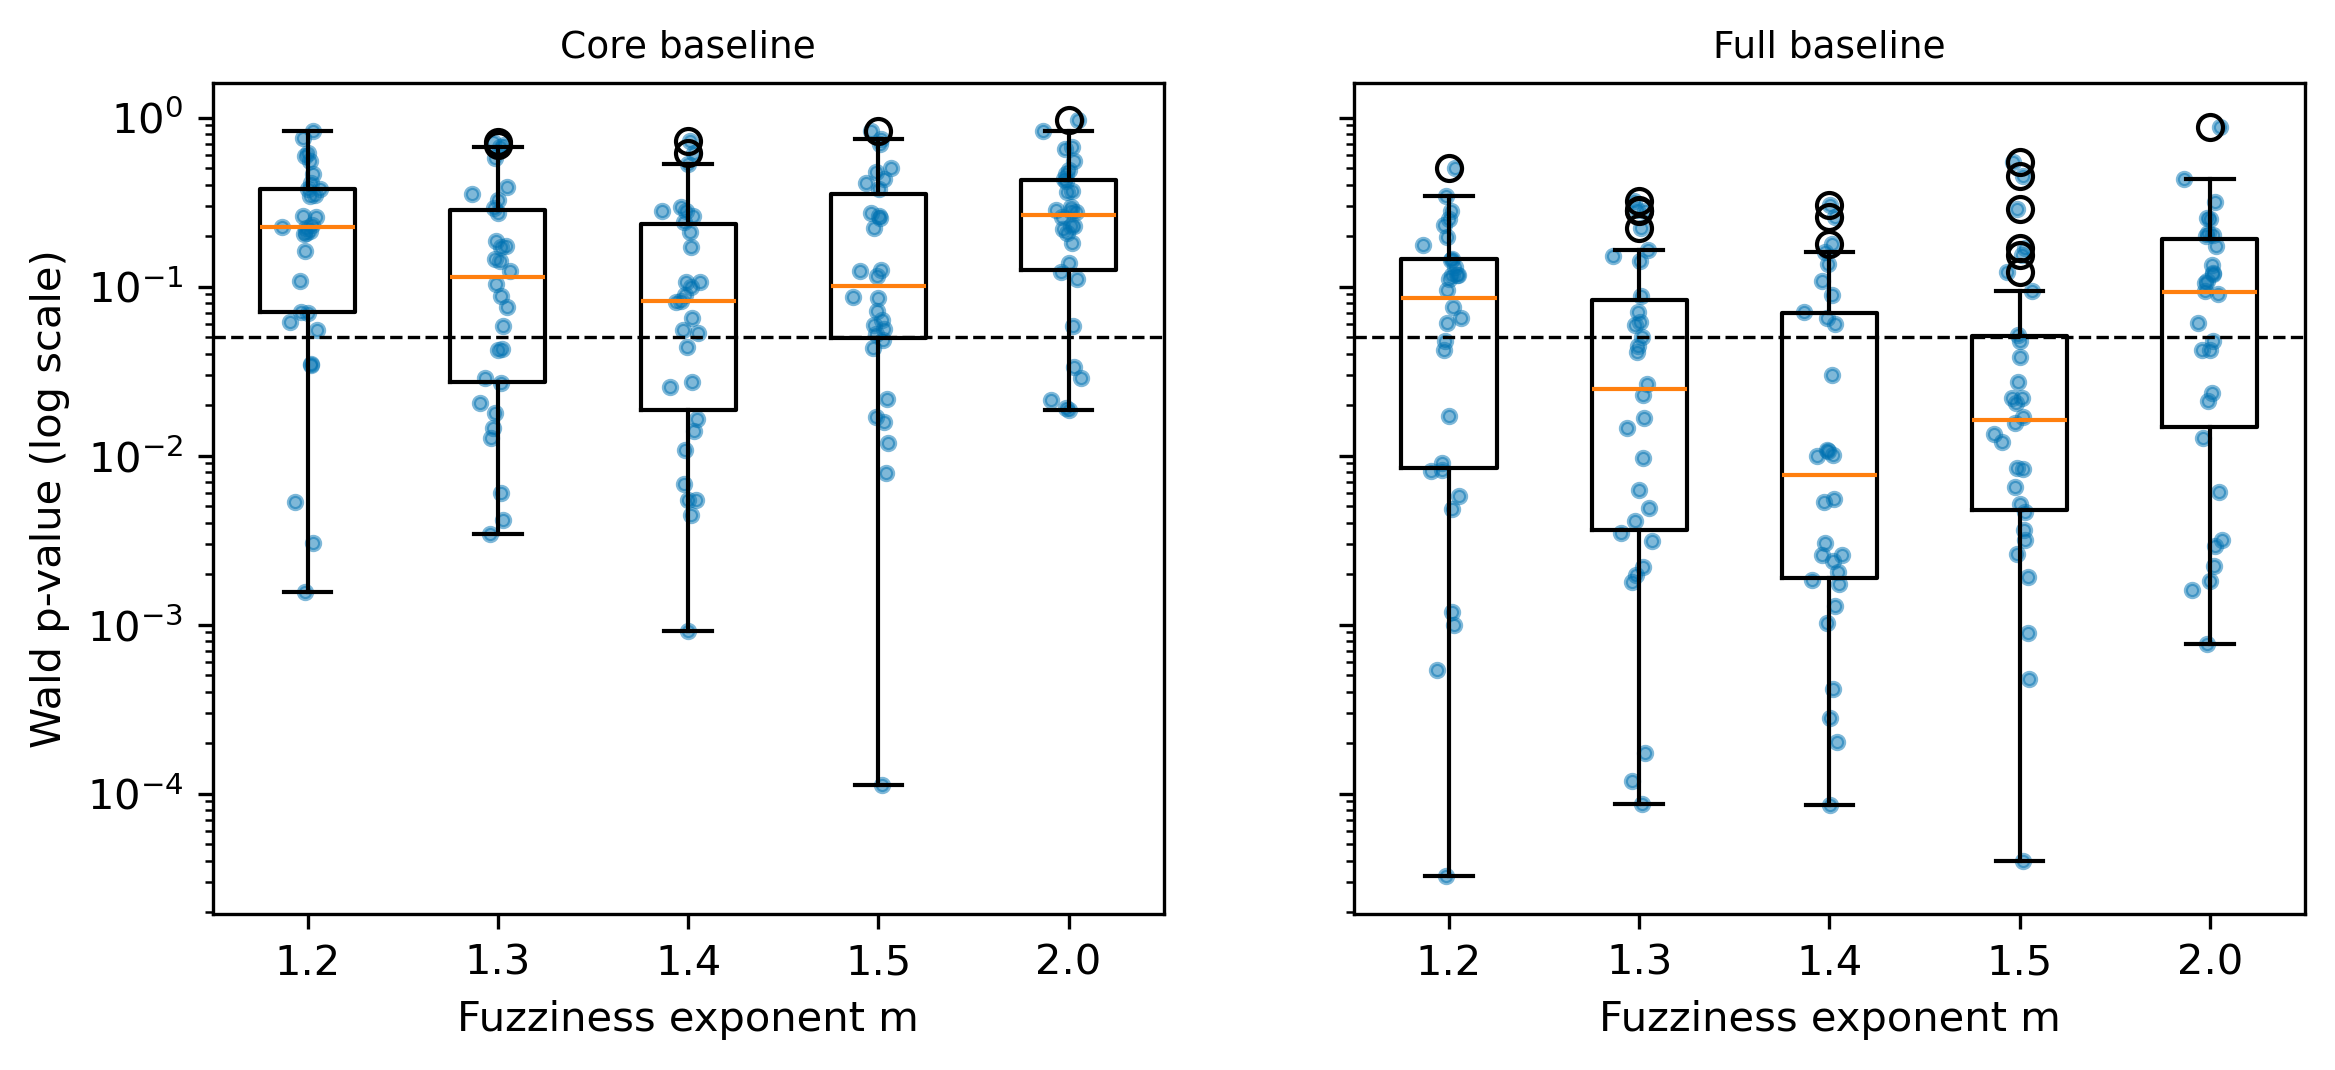
\includegraphics[width=0.85\textwidth]{thesis_outputs/figures/seed_sensitivity.png}
	\caption{Wald $p$-values over 30 random draws of the clustering, by fuzziness}
	\label{fig:seeds}
	\par\smallskip
	\parbox{0.9\textwidth}{\footnotesize\emph{Note.} Each point is one draw; boxes show the quartiles; the dashed line is $p=0.05$; the scale is logarithmic.}
\end{figure}

The $p$-values vary by orders of magnitude between draws: at $m=1.3$ the full-baseline $p$-value ranges from below 0.001 to 0.32 and the core-baseline value from 0.003 to 0.71. Against the full baseline, the test is significant in 60\% of the draws at $m=1.3$ (median $p=0.025$), 67\% at $m=1.4$ (0.008) and 73\% at $m=1.5$ (0.016), and in 40\% and 43\% at $m=1.2$ and $m=2.0$. Against the core baseline it is significant in 37\%, 37\% and 27\% of the draws at $m=1.3$, 1.4 and 1.5 (medians of 0.08 to 0.11). The median gain in adjusted $R^2$ is 0.26 to 0.38 percentage points against the full baseline and 0.10 to 0.14 points against the core baseline. Out of sample, the median gain is positive against the full baseline (0.12 to 0.23 points, with a positive gain in 70 to 77\% of the draws) but negative against the core baseline (between $-0.02$ and $-0.07$ points, positive in only 40 to 43\% of the draws). The run reported in Chapter~\ref{ch:results} is a favourable draw: its conventional $p$-values (0.027 and 0.002) are lower than the medians over draws (0.11 and 0.025) and its out-of-sample gains are larger. A typical draw therefore shows an association against the full baseline, but not an improvement in out-of-sample prediction over the core baseline, which is the better predictor (cross-validated $R^2$ of 0.436 against 0.422 for the full baseline). Against the full baseline, which overfits, the membership changes improve prediction in most draws; this is consistent with, but does not show, that they act partly as a regulariser for the twenty-four additional statistics.

\section{Estimated attribute weights}
\label{sec:rob-weights}

The estimation of the attribute weights, which the proposal envisaged, was tried first and abandoned (Section~\ref{sec:method-model}). Appendix~\ref{app:weights} reports the weights obtained for the 2023/24 season in the variants that were tried. They show that the failure is systematic and not specific to one setting: in the variants that avoid collapse onto the success rates, positions take most of the weight, and with five clusters the weights collapse onto the positions in all four variants.

\section{Summary}

The association between membership changes and changes in market value in the main configuration is robust to the definition of the sample and the outcome, to player fixed effects, and to the inclusion or exclusion of performance controls, and it is not reproduced by a linear summary of the same statistics. It depends on the clustering. It is absent for near-crisp memberships ($m=1.2$), for $K=5$ and, at $m=1.3$, for $K=3$ with shrunk rates, strongest at $m=1.4$ to $1.5$, and weaker when fewer players are assigned to the noise cluster. It varies greatly with the random draw of the clustering, in which it is found against the full baseline in about two thirds of the draws and against the core baseline in about a third, and in which the out-of-sample gain over the core baseline is typically absent. Applying a correction for the number of comparisons leaves no result significant. The evidence is therefore weak and specification-dependent: it points to a small association between the movement from the defender profile to the wide-attacker profile and changes in value, but not to a robust improvement in explanatory power.
